\documentclass{abstract_hutech}
\graphicspath{{images/}}
\usepackage{subcaption}
\begin{document}
\thispagestyle{firstpage}
\twocolumn[
\begin{@twocolumnfalse}
\vspace*{20pt}
\begin{flushleft}
\fontsize{20}{0}\selectfont{\textbf{천체망원경 모터 포커서 컨트롤러 구동 시스템 개발 및 ASCOM 드라이버 개발}}
\vspace{32pt}\par
\fontsize{10}{12}\selectfont{\textbf{본 논문에서는 자동 초점 조절 구동 시스템을 자동으로 구현하기 위한 방법을 제안한다. 자동 초점 조절 구동 펌웨어는 기본적으로 arduino를 사용하며 여러 기능들이 존재하여 자유로운 설정이 가능하다. ASCOM 드라이버는 C\# 코딩을 이용하여 컴퓨터로 정보전달이 가능하다. CCD 제어 프로그램은 카메라의 초점을 맞추기 위하여 어느 방향으로 돌려야 맞춰지는지를 확인한다. 본 논문에서 제안된 방법은 사람이 손으로 제어하는 것보다 정밀하고 빠르게 천체망원경의 초점을 맞출 수 있도록 편의성을 제공한다.
}}
\end{flushleft}
\vspace{20pt}
\end{@twocolumnfalse}
]

\section{서론}

\subsection{선정 배경}

%많은 사람들이 알고 있듯이 천체망원경으로 천체를 관측할 때 초점을 맞춘다면 관측할 천체의 모습이 더 선명하게 보인다. 그림 1의 (a)는 천체망원경의 초점을 맞추지 않고 천체망원경으로 찍은 사진이고, 그림 1의 (b)는 천체망원경의 초점을 맞추고 천체망원경으로 찍은 사진이다. 이 두 사진에서 볼 수 있듯이 초점을 맞췄을 때 천체가 더 선명하다는 사실을 알 수 있다. 하지만 Fig. \ref{fig:before} 에서의 사진도 작자의 손으로 초점을 맞춘 것이라 정확하게 초점이 맞지 않다. 또한 초점이 완벽하게 맞지 않았는데도 이러한 사진을 찍기 위해서 초점을 맞추는데 많은 시간을 투자해야 한다. 이렇듯 사진을 통하여 정밀한 천체의 사진이 필요한 경우 사람의 손으로는 무리가 있다. 이러한 문제를 해결하기 위한 해결방법으로는 자동 초점 조절 장치가 있다. 자동 초점 조절 장치가 현재 개발되어 있는 제품이 미국 Starizona 회사의 Micro touch이다. 이 제품은 자동 초점 조절 시스템이 구현이 잘 되어 있으나, 가격이 499달러로 부담이 있다. 따라서 이러한 자동 초점 조절 장치를 arduino 기반으로 제작한다면 천체망원경의 초점을 맞출 때 사람들에게 편의성을 제공하고 이전의 제품보다 값싸게 비슷한 기능을 구현하는 것이 가능해질 것이다.

천체망원경으로 사진 관측을 할 때 정확한 초점 조정은 사진의 품질에 영향을 미치는 요소 중의 하나이다. 태양 사진을 촬영하면서 초점을 조절하는 과정을 Fig. \ref{fig:before_after}에 나타내었다. 초점 조정시 어려운 점은 초점을 조정하기 위해  초점 조절노브에 손이 닿으면 진동이 발생하고, 그 진동이 사진의 품질에 영향을 준다. 또한 초점 조절시 손으로 돌리는 것은 미세한 조정을 하기에 어려움이 있다. 할 때 초점을 맞추고 천체망원경으로 찍은 사진이다. 다. 또한 초점이 완벽하게 맞지 않았는데도 이러한 사진을 찍기 위해서 초점을 맞추는데 많은 시간을 투자해야 한다. 이렇듯 사진을 통하여 정밀한 천체의 사진이 필요한 경우 사람의 손으로는 무리가 있다. 이러한 문제를 해결하기 위한 해결방법으로는 자동 초점 조절 장치가 있다. 자동 초점 조절 장치가 현재 개발되어 있는 제품이 미국 Starizona 회사의 Micro touch이다. 이 제품은 자동 초점 조절 시스템이 구현이 잘 되어 있으나, 가격이 499달러로 부담이 있다. 따라서 이러한 자동 초점 조절 장치를 arduino 기반으로 제작한다면 천체망원경의 초점을 맞출 때 사람들에게 편의성을 제공하고 이전의 제품보다 값싸게 비슷한 기능을 구현하는 것이 가능해질 것이다.

\begin{figure}[h]
\begin{subfigure}{0.45\linewidth}
\centering

\includegraphics[width=1\linewidth]{before}
\caption{초점을 맞추기 전}
\label{fig:before}
\end{subfigure}
\begin{subfigure}{0.45\textwidth}
\centering
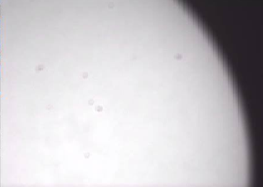
\includegraphics[width=1\linewidth]{after}
\caption{초점을 맞춘 후}
\label{fig:after}
\end{subfigure}
\caption{초점을 맞춘 사진과 맞추지 않은 사진의 비교}
\label{fig:before_after}
\end{figure}

\subsection{이론적 배경}

그림 \ref{fig:telescope1}가 바로 Micro touch로, 시중에 있는 자동 초점 조절 장치이다. 이를 옆의 컴퓨터와 연결시킨 그림이 바로 그림3으로, 이를 이용하여 컴퓨터에서도 ASCOM이라는 프로그램을 이용하여 원격으로 모터의 초점을 맞출 수 있도록 설정할 수가 있다. 그림2에서 나온 위의 두 버튼(IN, OUT)은 각각 초점을 맞추기 위해 망원경의 길이를 줄이거나 늘일 수 있는 버튼이다. Micro touch를 수동 혹은 자동으로 작동시켜 IN또는 OUT의 명령을 내렸을 경우, 그림 4에 보이는 모터포커서가 작동하게 된다. 이 모터포커서는 그림 4의 오른쪽에 보이는 모터를 움직여 천체망원경의 경통의 길이를 조절할 수 있도록 한다. 경통의 길이가 변화하면 그에 따라서 빛이 퍼지는 정도가 달라지므로 이를 잘 조정하면 망원경으로 관측하는 천체의 초점을 맞출 수 있게 된다.

\begin{figure}[h]
	\centering
	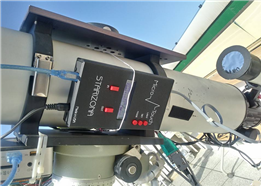
\includegraphics[width=1\linewidth]{telescope1}
	\caption{Micro Touch를 천체망원경에 부착시킨 모습}
	\label{fig:telescope1}
\end{figure}

\begin{figure}[h]
	\centering
	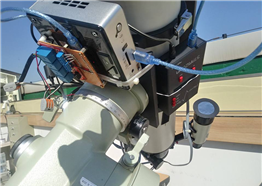
\includegraphics[width=1\linewidth]{telescope2}
	\caption{Micro Touch와 연결된 컴퓨터}
	\label{fig:telescope2}
\end{figure}

\begin{figure}[h]
	\centering
	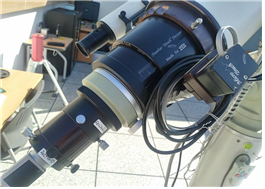
\includegraphics[width=1\linewidth]{telescope3}
	\caption{모터포커서와 망원경의 길이}
	\label{fig:telescope3}
\end{figure}

\subsection{선행연구 고찰}

이덕규 외(2014)는 복합재 광구조체와 결합하여 전자광학카메라의 영상품질을 향상시킬 수 있는 초점조절장치를 개발하였다.\cite{leedukgu2014}

윤종환 외(2011)는 선명도에 관한 기울기를 이용하여 초점이 맞았는지를 확인하는 방법을 사용하였다.\cite{yunjonghwan2011lcd}

박석휘 외(2009)는 모바일 폰용 자동 초점 조절 알고리즘을 초점 값 계산 알고리즘을 이용하여 구현하였다.\cite{parksukhui2009Median}

이성희 외(1998)는 각 화소들의 미디언 값의 차이를 이용하여 초점을 맞추는 알고리즘을 구현하였다.\cite{leeseonghee1998Median}


\section{개발 내용 및 방법}

\subsection{사용한 망원경}

TEC140 광학계에는 Starlight Instruments에서 제작한 3.5" Feather Touch Focuser가 장착 되어 있다. 
https://www.baader-planetarium.com/en/telescopes/tec/tec-apo-140-ed-triplet-apochromat.html 

Starlight Instruments에서는 3.5" Feather Touch Focuser에 장착할 수 있는 STEPPER MOTOR와 MICRO TOUCH FOCUSING SYSTEM을 제작하여 판매하고 있다. 
(참고사이트 : http://starlightinstruments.com/store/index.php?route=product/category&path=41)
(참고사이트 : http://starlightinstruments.com/store/index.php?route=product/product&path=41&product_id=90 )

모터는 구입한 것을 사용하고 MICRO TOUCH FOCUSING SYSTEM과 같은 기능을 가진 포커서 컨트롤러를 제작하였다.


\subsection{모터 포커서 컨트롤러 회로 설계}


사용한 부품의 리스트를 만들고 스펙과 설명을 넣자.

서킷 메이커 회로도 첨부 

만능기판으로 만든 사진 첨부

pcb 사진 첨부 및 pcb로 제작한 사진 첨부


\subsection{모터 포커서 구동 펌웨어 개발}

펌웨어에 들어간 기능들 넣고, 
코드에 대한 흐름도(flow chart) 넣으면 좋을듯.

자동 초점 조절을 위하여 가장 필요한 것이 모터를 돌리는 과정인데, 초점을 맞추기 위하여 모터를 돌리는 방향과 각도 또한 중요하다. 이를 arduino로 구현하고, 적절한 회로를 짜서 제대로 기능하는지 확인하고, 자동 초점 조절 장치에도 연결하여 수동적으로 초점 조절이 가능한지 확인한다. 천체망원경에 종류에 따라 모터를 돌려야 할 기준점이 다를 수 있으므로 기본 값 설정이 가능하게 하고, 컴퓨터와의 연동을 위한 블루투스 장치를 추가한다. 또한, 이전의 제품과 차별성을 부여하기 위하여 모터를 돌릴 때 가속기능을 추가하고, 천체망원경은 날씨에 민감하므로 온습도 센서를 추가한다.

\subsection{ASCOM 드라이버 개발 및 컴퓨터와 연동}

모터 자동 초점 조절 장치를 활용하기 위해서는 별의 크기를 분석해서 돌려야 하므로 컴퓨터와의 연동을 위하여 자동 초점 조절 장치의 ASCOM 드라이버를 C\# 코딩을 이용하여 제작한다. ASCOM 드라이버를 이용하면 카메라로부터 정보를 컴퓨터가 받아서 데이터를 분석하고, 이 분석한 데이터를 이용하여 모터를 어떻게 조절해야 할지 명령을 내리면 ASCOM 드라이버를 통해 정보를 전달하여 모터를 제어한 대로 조절이 가능하다.


\section{결론}

\subsection{연구결과의 활용과 기대효과}

자동 초점 조절 장치 없이 사람이 직접 초점을 맞추는 것은 정확하지 않고 시간이 많이 든다. 이를 해결하기 위해서 시중에 나온 Micro Touch의 경우 이러한 문제점들을 잘 해결해주고 있다. 하지만 가격이 비싸서 부담스러울 수 있고, 제품을 사용하다보면 길이를 늘이거나 줄일 때 가속기능이 존재하지 않아서 설정되어야 하는 값과 현재 값이 차이가 많이 난다면 설정하는데 시간이 오래 걸린다는 단점이 있다. 본 연구에서는 이러한 단점들을 보완하여 가속기능을 추가하고, arduino 코딩을 기반으로 자동 초점 조절 장치를 개발한다. 이러한 자동 초점 조절 장치가 이용된다면 현재보다 더욱 편리하게 천체망원경의 초점을 맞출 수 있게 되어 천체를 관측하거나 초점을 조절하여 찍은 사진을 이용하는 연구의 경우 사람의 손보다 수월하게 진행이 가능하다.

\subsection{추후 연구}

\subsubsection{카메라(또는 CCD) 제어 S/W 개발}

사진 관측을 이용해서 얻은 사진을 컴퓨터로 연결하여 분석이 가능할 수 있도록 만든 카메라(CCD) 제어 시스템을 개발한다. 이를 위하여 사진을 컴퓨터로 보낼 수 있어야 한다. 또한, 카메라에 나오는 화면의 변화를 보아야 하므로 연속적인 변화를 실시간으로 보낼 수 있는 프로그램을 만들어서 컴퓨터가 제대로 인식을 하여 모터에 올바른 명령을 내릴 수 있는지 확인한다.

\subsubsection{오토 포커싱 알고리즘 구현}

천체망원경의 초점을 맞추기 위해 사진 관측의 사진을 연속적으로 찍어서 컴퓨터로 보내주고, 컴퓨터는 이를 분석하여 자동 초점 조절 장치 컨트롤러에 별의 크기가 커지고 있는지 작아지고 있는지 정보를 알고리즘에 보내준다. 그러면 프로그래밍 된 arduino가 모터를 어느 방향으로 돌려야 하는지 판단하여 모터를 돌리고, 이 과정을 반복하여 별의 크기가 제일 작아질 때, 즉 별의 초점이 맞을 때 이 과정을 멈춘다. 이러한 과정이 일어나는지 실제로 천체망원경에 달아서 확인한다.


\bibliography{bibfile} % 참고문헌

\end{document}